%%%%%%%%%%%%%%%%%%%%%%%%%%%%%%%%%%%%%%%%%%%%%%%%%%%
% PHỤ LỤC
%%%%%%%%%%%%%%%%%%%%%%%%%%%%%%%%%%%%%%%%%%%%%%%%%%%
\section*{PHỤ LỤC}
\thispagestyle{empty}
\addcontentsline{toc}{section}{\numberline{}PHỤ LỤC}

\subsection*{Phụ lục A: Mã nguồn C++ thuật toán lọc tư thế và điều khiển PID (STM32)}

Dưới đây là đoạn mã nguồn C++ cốt lõi thực thi thuật toán bộ lọc bù (Complementary Filter) và tính toán PID kép (Cascade PID) cho góc tư thế trong vòng lặp điều khiển bay chính:

\begin{lstlisting}[language=C++]
// Cap nhat bo loc bu (Complementary Filter) de tinh toan goc Roll, Pitch
void calculateAttitude(float ax, float ay, float az, float gx, float gy, float gz, float dt) {
    // Tinh toan goc nghieng tuyet doi tu Accelerometer
    float roll_acc = atan2(ay, az) * 180.0 / M_PI;
    float pitch_acc = atan2(-ax, sqrt(ay * ay + az * az)) * 180.0 / M_PI;

    // Tinh phan tram ket hop: 98% Gyroscope va 2% Accelerometer
    float alpha = 0.98f;
    current_roll = alpha * (current_roll + gx * dt) + (1.0f - alpha) * roll_acc;
    current_pitch = alpha * (current_pitch + gy * dt) + (1.0f - alpha) * pitch_acc;
}

// Bo dieu khien PID roi rac cho tung truc bay
float calculatePID(float setpoint, float feedback, PID_Config &cfg, float dt) {
    // 1. Tinh error
    float error = setpoint - feedback;
    
    // 2. Khau ti le (Proportional)
    float p_out = cfg.Kp * error;
    
    // 3. Khau tich phan (Integral) co chong bao hoa (Anti-windup clamping)
    cfg.i_mem += cfg.Ki * error * dt;
    if (cfg.i_mem > cfg.i_max) cfg.i_mem = cfg.i_max;
    else if (cfg.i_mem < -cfg.i_max) cfg.i_mem = -cfg.i_max;
    
    // 4. Khau vi phan (Derivative) qua bo loc thong thap IIR
    float d_raw = (error - cfg.last_error) / dt;
    cfg.last_error = error;
    
    // Loc thong thap IIR bac 1 cho khau vi phan
    cfg.d_filtered = cfg.d_filtered * 0.7f + d_raw * 0.3f;
    float d_out = cfg.Kd * cfg.d_filtered;
    
    // Tong gia tri dau ra
    float output = p_out + cfg.i_mem + d_out;
    return output;
}
\end{lstlisting}

\subsection*{Phụ lục B: Mã nguồn Python thuật toán phát hiện cử chỉ vẫy tay cầu cứu}

Đoạn mã Python dưới đây thực thi thuật toán phân tích 17 keypoints của YOLOv8-Pose để phát hiện cử chỉ vẫy hai tay cầu cứu tuần hoàn của nạn nhân tại trạm mặt đất:

\begin{lstlisting}[language=Python]
import numpy as np

class GestureAnalyzer:
    def __init__(self, window_size=30):
        self.window_size = window_size
        self.history = []  # Luu tru chuoi keypoints
        self.threshold_wave = 0.15 # Nguong bien do dao dong

    def update(self, keypoints):
        """
        keypoints: mang numpy shape (17, 3) chua toa do [x, y, confidence]
        """
        self.history.append(keypoints)
        if len(self.history) > self.window_size:
            self.history.pop(0)

        if len(self.history) < self.window_size:
            return False

        # 1. Trich xuat toa do y cua vai va co tay cua cac khung hinh trong hang doi
        left_shoulders_y = [kp[5][1] for kp in self.history]
        right_shoulders_y = [kp[6][1] for kp in self.history]
        left_wrists_y = [kp[9][1] for kp in self.history]
        right_wrists_y = [kp[10][1] for kp in self.history]
        left_wrists_x = [kp[9][0] for kp in self.history]
        right_wrists_x = [kp[10][0] for kp in self.history]

        # 2. Tinh toan chieu dai than nguoi trung binh lam he so chuan hoa
        torso_lengths = [np.linalg.norm(kp[5][:2] - kp[11][:2]) for kp in self.history]
        avg_torso = np.mean(torso_lengths) if np.mean(torso_lengths) > 0 else 1.0

        # 3. Kiem tra co tay co cao hon vai hay khong (y_wrist < y_shoulder)
        hands_up_left = all(y_w < y_s for y_w, y_s in zip(left_wrists_y, left_shoulders_y))
        hands_up_right = all(y_w < y_s for y_w, y_s in zip(right_wrists_y, right_shoulders_y))

        if not (hands_up_left and hands_up_right):
            return False

        # 4. Phan tich tan so va bien do dao dong truc ngang (X) cua co tay
        std_x_left = np.std(left_wrists_x) / avg_torso
        std_x_right = np.std(right_wrists_x) / avg_torso

        # Dem so lan doi huong de xac dinh tinh tuan hoan
        diff_left = np.diff(left_wrists_x)
        directions_left = np.sign(diff_left)
        direction_changes = np.sum(np.diff(directions_left) != 0)

        # Dieu kien xac nhan vay tay
        if (std_x_left > self.threshold_wave and 
            std_x_right > self.threshold_wave and 
            direction_changes >= 4):
            return True
        return False
\end{lstlisting}

\subsection*{Phụ lục C: Bản vẽ sơ đồ mạch nguyên lý Flight Controller và Layout PCB}

Dưới đây là hình ảnh minh họa bản vẽ thiết kế nguyên lý tổng thể của bo mạch điều khiển bay và đường đi dây Layout PCB 2 lớp:

\begin{figure}[H]
    \centering
    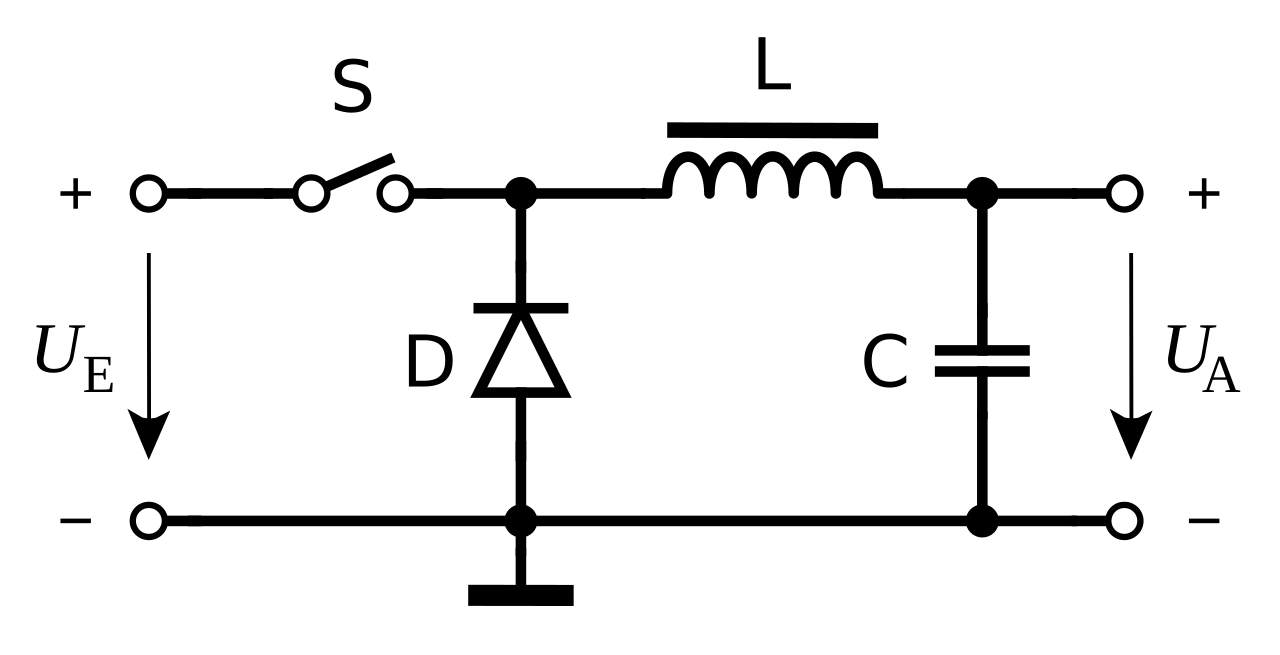
\includegraphics[width=0.95\textwidth]{Images/agent/mach_nguon_lm2596_ams1117.png}
    \caption[Sơ đồ thiết kế mạch in PCB Flight Controller hai lớp]{\bfseries\fontsize{12pt}{0pt}\selectfont Sơ đồ thiết kế mạch in PCB Flight Controller hai lớp}
    \label{fig:layout_pcb_full}
\end{figure}
